\documentclass{soil12}
\pagesettings
\title{Construction of Auditorium Building at Baba Banda Bahadur College of Nursing, Faridkot}


\begin{document}
\maketitle
\clearpage

\heading{GURU NANAK DEV ENGINEERING COLLEGE, LUDHIANA}
{Accredited by NBA (AICTE), New Delhi (ISO 9001:2000 Certified)}
{Testing \& Consultancy Cell }
{tcc@gndec.ac.in }
{0161-2491193}
\sethead{List of Faculty/Experts}
\listdata{Geotechnical}{Dr. J.N.Jha, Ph.D\\
Prof. Kulbir Singh Gill,M.E\\
Dr. B.S.Walia, Ph.D.\\
Prof. Harjinder Singh, M.E\\
Prof. Gurdeepak Singh, M.Tech.\\
}
\listdata{Structure}{Dr. Harpal Singh, Ph.D\\
Dr. Hardeep Singh Rai, Ph.D\\
Prof. Harvinder Singh, M.Tech\\
Dr. Jagbir Singh, Ph.D.\\
Prof. Kanwarjit Singh Bedi, M.Tech.\\
Prof. Parshant Garg, M.Tech\\
Prof. Harpreet Kaur, M.Tech.\\
Prof. Inderpreet Kaur, M.Tech.
}

\listdata{Highway}{Prof. Kulbir Singh Gill, M.E\\}
\listdata{Material Testing}{Dr. Jagbir Singh, Ph.D.\\
Prof. Kanwarjit Singh Bedi, M.Tech.\\
}

\listdata{Material Testing}{Dr. Jagbir Singh, Ph.D.\\
Prof. Kanwarjit Singh Bedi, M.Tech.\\
}

\listdata{Survey}{Dr. B.S.Walia, Ph.D.\\
}

\listdata{Chemical Testing}{Dr. R.P.Singh, Ph.D.\\
}

\listdata{Environmental Engg}{Prof. Puneet Pal Singh, M.E\\
}
\clearpage
\reportheading{SOIL INVESTIGATION REPORT}
\begin{enumerate}
\item{
\reportdetail{Date of Testing}{13.04.2011}}
\item{\reportdetail{Type of Structure}{Building}}
\item{\reportdetail{Site location}{Latitude : 31.4177 Longitude : 75.9539}}
\item{\reportdetail{Map}{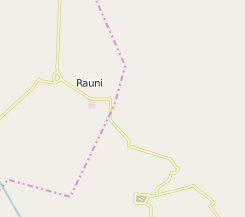
\includegraphics[scale=0.3]{map.png}}}

\item{\reportdetail{Tested in Presence of}{Sh. Puneet Inder Bawa, Chairman\\
 Sh. Ramesh Kumar, Superwiser}}
\item{\reportdetail{Report Submitted to}{Sh. Puneet Inder Bawa, Chairman\\
 Sh. Ramesh Kumar, Superwiser}}
\item{\reportdetail{Report Prepared by}{Dr. J. N. Jha\\
Prof. Kulbir Singh Gill\\
 Dr. B. S. Walia}}
\end{enumerate}
\clearpage
\section{Introduction}
The soil investigation for the proposed Construction of Auditorium Building at Baba Banda Bahadur
College of Nursing, Faridkot had been taken up on request of Chairman, Baba Banda Bahadur
College of Nursing, Vire Wala Road, Faridkot. The field soil investigation as per requirements was
carried out on 13.04.2011 by testing team of this institution in the presence of Sh. Puneet Inder Bawa,
Chairman, Sh. Ramesh Kumar, Superwiser of the concerned department.\par
The purpose of this soil investigation was to determine the nature of the subsoil stratum and the safe net
allowable bearing capacity of the soil.

\section{Field Soil Investigation}
Three bore holes were tested in the field Standard Penetration Test (S.P.T) was carried out at the proposed
site as per I.S.Code 2131-1981 in the soil deposits at the foundation level and at an interval of 1.5 m or at
the location where change of soil strata takes place during field testing. The samples of the soil both
disturbed and tube samples were collected at different depths and were properly sealed in air-tight plastic
bags after labelling them carefully to maintain the natural moisture content.
\section{Laboratory Testing}
As per I.S. Code 6403-1981, the least of the following shall be taken as safe net allowable bearing
capacity of the soil.
\begin{enumerate}
\item{The safe net allowable bearing capacity from shear considerations is obtained by dividing net
ultimate bearing capacity by a suitable factor of safety.}
\item{The safe net allowable bearing pressure that can be imposed on the base of the foundation
without the settlement exceeding a permissible value is calculated either from settlement
analysis or from the Standard Penetration Test Values(N)whichever is applicable depending
upon the nature of sub soil strata.}
\end{enumerate}
\section{Water Table}
The underground (i.e. sub-soil) water was encountered at a depth 0.6 m at the time of field soil
investigation.
\section{Proposed Substructure}
The substructures i.e. foundations of the proposed Building may be taken as wall footing and isolated
column foundation. The least soil properties have been taken for calculating the bearing capacity of
soil for the following types of foundations.
\begin{enumerate}
\item{\large{\textbf{Wall Foundation}}}\\
\wallfound{2}{3}
\item{\large{\textbf{Column Foundation}}}\\
\colfound{3m}{4.5m}{3.5m}{3.5m}{3.5m}
\end{enumerate}
The data obtained from the field soil investigation and the laboratory tests have been used in the
preparation of this report.
\section{Bearing Capacity Calculations}
\subsection{Bearing Capacity Based on Shear Considerations}
(As per I.S.Code - 6403:1981)
\subsection{Wall Foundation}
\wallfound{3.5m}{3.0m}

The least soil properties at the foundation level i.e. at 3.5 m depth are:\\
\soilproperty{2}{4}{5}{6}

Bearing Capacity factors are:\\
\bearingcapacity{15.3}{15.4}{16.4}
Shape factors are:\\
\shapefactor{3.3}{4.3}{3.3}
Depth factors are:\\    
\depth{3}{4}
Water table correction factor, w' = 0.5

Ultimate net bearing capacity, $q_u$' = 0.67 x0.5 x15.26 x1.3 x1.38 +17.66 x3.5 x(1 -6.72) x1.3 x1.19 +0.5 x17.66 x3.0 x5.79 x1.3 x1.19 x0.5\\
= 9.03 +504.87 +73.0 = 586.90 kN/$m^2$ \\	
Safe net allowable bearing capacity = $q_u'$/2.5 = 586.90/2.5 = 234.76 kN/$m^2$
\subsection{Column Foundation}
\colfound{3}{4}{5}{5}
The least soil properties at the foundation level i.e. at 3.5 m depth are: \\
\soilproperty{3}{4}{5}{5}
Bearing Capacity factors are:\\
\bearingcapacity{3}{5}{6    }
Shape factors are:\\
\shapefactor{4}{5}{6}
Depth factors are:
\depth{4}{5}
Water table correction factor, w' = 0.5 \\
Ultimate net bearing capacity, $q_u'$ = 0.67 x0.5 x15.26 x x +17.66 x3.5 x(1 -6.72) x x 
+0.5 x17.66 x3.0 x5.79 x x x0.5\\
= kN/$m^2$ = Safe net allowable bearing capacity = q\textsubscript{u} '/2.5 = /2.5 = kN/$m^2$
\section{Bearing Capacity Based on Standard Penetration Test Value}

\begin{center}
The result of concrete cubes sent by you tested on 29.10.11 are as under:
\end{center}
\hspace{1.1cm}
\begin{tabularx}{\textwidth}{|*{6}{l|}}
\hline
 \multicolumn{1}{|m{1cm}|}{Sr No.} &\multicolumn{1}{m{2cm}|}{Depth(m)} &\multicolumn{1}{m{2.5cm}|}{Overburden pressure (kN/m\textsuperscript{2})}
&\multicolumn{1}{m{2cm}|}{Correction Factor} &\multicolumn{1}{m{2cm}|}{Observesd Value of N} &\multicolumn{1}{m{2.9cm}|}{Corrected Value of N}\\
\hline
1 &3.5 &29 &1.36 &03 &04.80\\
\hline
1 &3.5 &29 &1.36 &03 &04.80\\
\hline
1 &3.5 &29 &1.36 &03 &04.80\\
\hline
1 &3.5 &29 &1.36 &03 &04.80\\
\hline
1 &3.5 &29 &1.36 &03 &04.80\\
\hline
1 &3.5 &29 &1.36 &03 &04.80\\
\hline
\end{tabularx}

\begin{enumerate}
\item{\standardvalue{4}{5}{6}{4}{3}{3}{4}{3}{5}}
\item{
\standardvalue{4}{5}{6}{4}{3}{3}{4}{3}{5}}
\end{enumerate}
\clearpage
\section{Remarks:}
\remark{4}{5}{6}{8}{9}
\footer{(Dr. B. S. Walia)\\
Associate Professor\\
Civil Engg. Department}{(Prof. Kulbir Singh Gill)\\
Associate Professor\\
Civil Engg. Department}

\footer{(Dr. J. N. Jha)\\
H.O.D., Civil Engg. Department}{(Dr. H. S. Rai)\\
Dean Testing \& Consultancy
    }
\end{document}

